% SPDX-License-Identifier: AGPL-3.0-or-later
% Commercial license available
% © Concepts 1996-2026 Miroslav Sotek. All rights reserved.
% © Code 2020-2026 Miroslav Sotek. All rights reserved.
% ORCID: 0009-0009-3560-0851
% Contact: www.anulum.li | protoscience@anulum.li
% scpn-quantum-control --- S1 monitored-feedback control short paper

\documentclass[preprint,aps,physrev,superscriptaddress,floatfix,longbibliography]{revtex4-2}

\usepackage{amsmath,amssymb}
\usepackage{booktabs}
\usepackage{graphicx}
\usepackage{hyperref}
\usepackage{xcolor}
\usepackage{xurl}
\usepackage{siunitx}

\hypersetup{
    colorlinks=true,
    linkcolor=blue!60!black,
    citecolor=blue!60!black,
    urlcolor=blue!60!black,
}

\begin{document}
\emergencystretch=3em

\title{Monitored feedback versus open-loop control for Kuramoto--XY synchronisation on IBM dynamic circuits}

\author{Miroslav \v{S}otek}
\email{protoscience@anulum.li}
\affiliation{ANULUM, Marbach SG, Switzerland}
\affiliation{ORCID: 0009-0009-3560-0851}

\date{May 20, 2026}

\begin{abstract}
Dynamic circuits make it possible to test monitored quantum-control policies
on gate-model hardware rather than only static circuit families. We report a
preregistered four-qubit Kuramoto--XY feedback experiment on
\texttt{ibm\_kingston}. The payload uses three system qubits, one monitor
qubit, three dynamic rounds, and paired hardware arms: a monitored-feedback
arm and a matched open-loop control. The preregistered binary synchronisation
endpoint is negative: the feedback arm gives mean target error 0.2148958333,
while the matched control gives 0.2116406250, so the feedback policy does not
improve the selected target. Because the binary proxy is near saturation in
both arms, we add same-paper direct-observable extensions. S1b measures final
XY-sector correlators on the original body; S1c reduces depth and gain; S1d
and S1e sweep and repeat policy direction; and S1f tests quadrature and
population controls. The extensions expose structured, policy-sensitive
feedback--control differences, including a repeated positive \texttt{YYI}
response in one shallow policy window. A later quadrature check does not
reproduce that large \texttt{YYI} response, reducing the mean absolute
feedback--control separation to 0.0082812500 and blocking a stable
controller-promotion claim. The contribution is therefore a hardware-control
boundary result: paired dynamic-circuit feedback tests and direct Pauli
readouts can reveal calibration-window-sensitive response modes, but the
tested controller is not supported as a backend-general or robust
synchronisation-improving policy.
\end{abstract}

\maketitle

\section{Introduction}

Kuramoto synchronisation is a canonical model for collective phase dynamics
and has a long history in nonlinear science~\cite{Kuramoto1975,Acebron2005}.
Gate-model quantum circuits can encode small XY-type phase-coupled systems,
but noisy intermediate-scale quantum hardware requires conservative claim
boundaries~\cite{Preskill2018,NielsenChuang2010}. In this setting, the
scientific question is not whether a broad quantum advantage has been shown.
The useful question is narrower: can a small monitored feedback policy improve
a preregistered hardware observable relative to a matched open-loop arm under
the same backend, layout, shot budget, repetitions, and calibration window?

Measurement-conditioned feedback is a standard quantum-control primitive
~\cite{WisemanMilburn2010}. Dynamic circuits provide the required gate-model
hardware surface: mid-circuit measurement, classical conditioning, and
subsequent gates within one submitted payload
~\cite{Corcoles2021,IBMQuantum,Qiskit2024}. Mid-circuit readout has also
become a practical resource for near-term quantum simulation
~\cite{Koh2023}, and adaptive circuits can express tasks unavailable to
fixed-depth unitary circuits at the same depth~\cite{FossFeig2023}. They also
create a stricter experimental standard. A feedback arm alone is not
interpretable, because backend drift, layout selection, readout bias, and
ordinary shot noise can all masquerade as control response. The S1 experiment
therefore uses a paired-arm design: every feedback run is compared with a
matched open-loop control generated from the same circuit body and executed in
the same hardware window.

This paper reports the completed S1 hardware programme. The primary
preregistered binary proxy is negative. The same-paper extensions then ask
whether the negative proxy hides smaller channel-level responses in direct
XY-sector observables. The final result is scientifically useful, but
conservative: the tested controller is not promoted. Instead, the paired-arm
method identifies a structured failure and sensitivity boundary for future
redesigned feedback policies.

\section{Preregistered S1 protocol}

The primary S1 payload uses three system qubits and one monitor qubit. The
feedback arm runs three dynamic rounds. In each round, the monitor qubit is
coupled to the system, measured, unconditionally reset, and used to condition a
small correction on the system. The matched open-loop arm preserves the same
body structure without using the measured monitor outcome as an active
feedback signal. The readiness artefact is generated by the committed S1
readiness script, and the canonical preregistration package is the JSON file
dated May 6, 2026 under \path{data/s1_feedback_loop/}.
The live payload used unconditional monitor reset and conditional correction
only, because the submitted provider path rejected reset operations inside
conditional blocks. This implementation detail is part of the experimental
boundary: the circuit tests provider-supported dynamic-circuit feedback, not
arbitrary low-latency real-time control.

\begin{table}[tb]
\centering
\begin{tabular}{lr}
\toprule
Protocol field & Value \\
\midrule
System qubits & 3 \\
Monitor qubits & 1 \\
Classical bits & 6 \\
Dynamic rounds & 3 \\
Hardware arms & feedback, matched open-loop control \\
Primary circuits & 2 \\
Shots per circuit & 1024 \\
Repetitions per arm & 12 \\
Target synchronisation proxy & 0.72 \\
\bottomrule
\end{tabular}
\caption{Primary S1 preregistered dynamic-circuit payload.}
\label{tab:protocol}
\end{table}

The primary endpoint is the absolute target-order-parameter error,
\begin{equation}
    \epsilon_{\mathrm{target}} = |R_{\mathrm{live}} - R_{\mathrm{target}}|,
\end{equation}
where $R_{\mathrm{target}}=0.72$. The feedback arm is useful under the
preregistered decision rule only if it reduces this error relative to the
matched open-loop control.

\section{Direct-observable extensions}

The primary binary proxy saturates near one on the selected backend. To avoid
over-interpreting a single nearly saturated readout, S1 includes a series of
same-paper direct-observable extensions. These are not separate papers and do
not change the primary endpoint. They localise the failure mode by measuring
XY-sector and control observables from matched feedback/control arms.

S1b preserves the original dynamic feedback body and measures final
\texttt{IXX}, \texttt{IYY}, \texttt{XXI}, and \texttt{YYI} correlators.
S1c reduces the body to one dynamic round, correction angle 0.06, and base
gain 0.4. S1d compares three preregistered one-round policy variants:
\texttt{current\_shallow\_positive}, \texttt{polarity\_flipped}, and
\texttt{weak\_positive}. S1e repeats that policy sweep at five repetitions per
arm. S1f keeps the S1d/S1e-favoured shallow policy and measures \texttt{XXI},
\texttt{XYI}, \texttt{YXI}, \texttt{YYI}, and \texttt{ZZI}. The
\texttt{XYI}/\texttt{YXI} rows test cross-quadrature leakage, while
\texttt{ZZI} is a population-sector control.

Figure~\ref{fig:s1-heatmap} gives the extension-level summary. The figure is
intended to expose the same logic as the tables: S1b is mixed-sign, S1c is
uniformly negative, the S1d/S1e current shallow policy has a narrow
\texttt{YYI} response, and S1f removes the stable positive-mechanism
interpretation in the later quadrature check.

For an observable $P$, each arm expectation is reduced from counts as
\begin{equation}
    \langle P \rangle =
    \frac{1}{N}\sum_b n_b \prod_{i\in \mathrm{supp}(P)}(-1)^{b_i},
\end{equation}

\begin{figure}[tb]
\centering
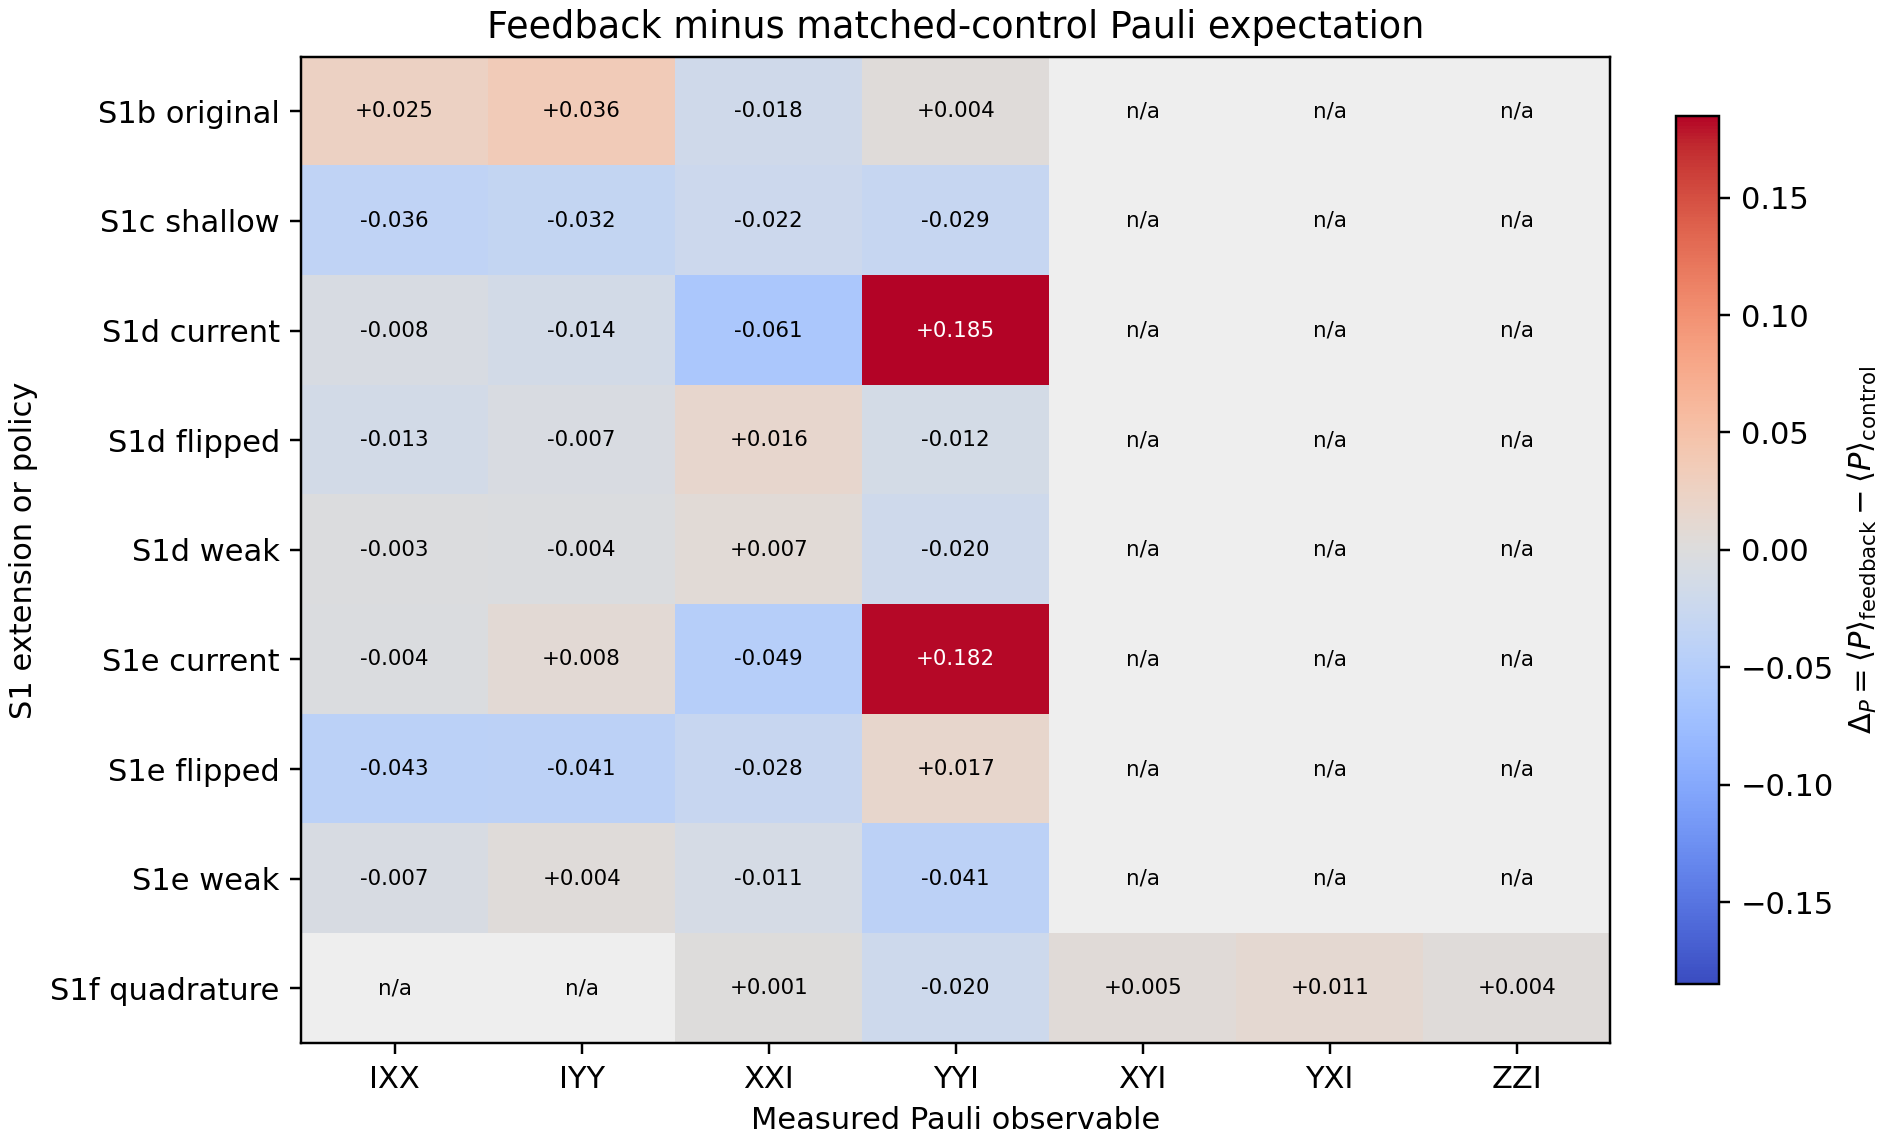
\includegraphics[width=0.98\linewidth]{../../figures/s1_feedback_control/s1_feedback_delta_heatmap_2026-05-20.png}
\caption{Feedback-minus-control Pauli expectations across the S1 direct
observable extensions. Grey cells mark observables not included in that
extension. The repeated S1d/S1e \texttt{YYI} response and the later S1f
sign reversal are visually isolated.}
\label{fig:s1-heatmap}
\end{figure}
with $n_b$ the observed count for bitstring $b$ and $N$ the total shots. The
reported extension quantity is
\begin{equation}
    \Delta_P =
    \langle P\rangle_{\mathrm{feedback}} -
    \langle P\rangle_{\mathrm{control}}.
\end{equation}

\section{Primary S1 result}

The primary paired-arm execution completed on \texttt{ibm\_kingston}. The
feedback job was \texttt{d86qn3lg7okc73elg2eg}; the matched open-loop control
job was \texttt{d86qn65g7okc73elg2hg}. Each arm used 12 repetitions and
12,288 total shots. The transpiled depths were 717 for the feedback arm and
684 for the matched control.

\begin{table}[tb]
\centering
\begin{tabular}{lrr}
\toprule
Metric & Feedback & Matched control \\
\midrule
Mean $R_{\mathrm{live}}$ & 0.9348958333 & 0.9316406250 \\
Mean target error & 0.2148958333 & 0.2116406250 \\
Final $R_{\mathrm{live}}$ & 0.9322916667 & 0.9322916667 \\
\bottomrule
\end{tabular}
\caption{Primary S1 binary-proxy hardware result on \texttt{ibm\_kingston}.}
\label{tab:s1-primary}
\end{table}

The feedback arm has a slightly larger mean synchronisation proxy than the
matched control, but both arms lie above the target. Consequently the feedback
arm is farther from the target. The target-error improvement is
$-0.0032552083$, corresponding to a relative improvement of
$-1.5380829334\%$. The preregistered decision is therefore
\texttt{null\_or\_negative}. This is the first claim boundary of the paper:
the tested three-round feedback payload does not improve the selected
binary-phase synchronisation proxy on this backend and calibration window.

\section{XY-sector localisation}

S1b asks whether the negative binary endpoint hides channel-level differences
in direct XY-sector observables. The original dynamic feedback body is
preserved, but the final basis is rotated to the selected Pauli correlator.
The results are shown in Table~\ref{tab:s1bc}.

\begin{table}[tb]
\centering
\begin{tabular}{lrr}
\toprule
Observable & S1b $\Delta_P$ & S1c $\Delta_P$ \\
\midrule
\texttt{IXX} & 0.0247395833 & -0.0364583333 \\
\texttt{IYY} & 0.0358072917 & -0.0319010417 \\
\texttt{XXI} & -0.0175781250 & -0.0221354167 \\
\texttt{YYI} & 0.0039062500 & -0.0292968750 \\
\midrule
Mean $|\Delta_P|$ & 0.0205078125 & 0.0299479167 \\
\bottomrule
\end{tabular}
\caption{S1b direct XY-sector extension and S1c shallow/gain-tuned extension.
S1b is mixed-sign; S1c is negative in all four channels.}
\label{tab:s1bc}
\end{table}

S1b is not a positive controller result. Three channels move in the feedback
direction and one moves against it, with mean absolute separation only
0.0205078125. It is, however, more informative than the saturated binary
proxy: the feedback/control difference is channel-structured rather than
uniformly absent.

S1c then tests whether the depth and gain of the original dynamic body are the
problem. The shallower, lower-gain policy reduces the feedback depths to about
237, but all four XY-sector channels move negative. The direct-observable
response therefore cannot be rescued by this shallow/gain-tuned policy.

\section{Policy-direction sweep and repeat}

S1d compares three one-round policy variants. S1e repeats the same policy
sweep at five repetitions per arm. The purpose is to distinguish a genuine
policy-direction response from a single noisy calibration window. The results
are shown in Table~\ref{tab:s1de}. The artefact timestamps place S1d at
13:46:14Z and S1e at 14:09:19Z on May 20, 2026, a separation of about
23 minutes under the same backend family and day.

\begin{table*}[tb]
\centering
\scriptsize
\begin{tabular}{@{}llrrrrrr@{}}
\toprule
Run & Variant & \texttt{IXX} & \texttt{IYY} & \texttt{XXI} & \texttt{YYI} & Mean signed & Mean abs. \\
\midrule
S1d & \texttt{current\_shallow\_positive} & -0.007813 & -0.013672 & -0.060547 & 0.184896 & 0.025716 & 0.066732 \\
S1d & \texttt{polarity\_flipped} & -0.013021 & -0.006510 & 0.015625 & -0.012370 & -0.004069 & 0.011882 \\
S1d & \texttt{weak\_positive} & -0.002604 & -0.003906 & 0.006510 & -0.020182 & -0.005046 & 0.008301 \\
\midrule
S1e & \texttt{current\_shallow\_positive} & -0.003516 & 0.008203 & -0.048828 & 0.182422 & 0.034570 & 0.060742 \\
S1e & \texttt{polarity\_flipped} & -0.042969 & -0.040625 & -0.028125 & 0.016797 & -0.023730 & 0.032129 \\
S1e & \texttt{weak\_positive} & -0.007422 & 0.004297 & -0.010547 & -0.040625 & -0.013574 & 0.015723 \\
\bottomrule
\end{tabular}
\caption{S1d policy-direction sweep and S1e higher-repetition repeat. Values
are feedback-minus-control Pauli expectations.}
\label{tab:s1de}
\end{table*}

The same narrow feature appears in both S1d and S1e:
\texttt{current\_shallow\_positive} has a large positive \texttt{YYI}
separation, 0.1848958333 in S1d and 0.1824218750 in S1e. The alternative
policies remain close to zero or negative by mean signed separation. This is a
real policy-sensitive signal candidate, but it is too narrow for controller
promotion: \texttt{IXX} and \texttt{XXI} remain negative for the same policy,
and the favourable aggregate is driven by one channel.

\section{Quadrature mechanism check}

S1f is the final same-paper discriminator. It keeps
\texttt{current\_shallow\_positive} and tests whether the repeated
\texttt{YYI} response belongs to a stable quadrature structure. It measures
the original \texttt{XXI}/\texttt{YYI} pair, the cross-quadrature controls
\texttt{XYI}/\texttt{YXI}, and a population control \texttt{ZZI}. The result
is shown in Table~\ref{tab:s1f}. Its artefact timestamp is 14:22:13Z, about
13 minutes after S1e and about 103 minutes after the primary S1 paired-arm
timestamp. This is therefore a later same-day calibration-window check, not a
multi-day stability claim.

\begin{table}[tb]
\centering
\begin{tabular}{lrrr}
\toprule
Observable & Feedback & Control & $\Delta_P$ \\
\midrule
\texttt{XXI} & 0.2187500000 & 0.2175781250 & 0.0011718750 \\
\texttt{XYI} & 0.1617187500 & 0.1566406250 & 0.0050781250 \\
\texttt{YXI} & 0.2242187500 & 0.2136718750 & 0.0105468750 \\
\texttt{YYI} & -0.0445312500 & -0.0242187500 & -0.0203125000 \\
\texttt{ZZI} & 0.6523437500 & 0.6480468750 & 0.0042968750 \\
\midrule
Mean $|\Delta_P|$ & \multicolumn{2}{r}{ } & 0.0082812500 \\
\bottomrule
\end{tabular}
\caption{S1f quadrature and population-control check. The large positive
\texttt{YYI} response seen in S1d/S1e does not persist in this later window.}
\label{tab:s1f}
\end{table}

The S1f result blocks the strongest possible positive interpretation of S1d
and S1e. The \texttt{YYI} separation changes sign and the mean absolute
feedback--control separation falls to 0.0082812500. The cross-quadrature
controls are small, and the population control is also small. The conservative
interpretation is calibration-window-sensitive response, not a stable
quadrature-localised feedback mechanism.

\section{Reproducibility artefacts}

The hardware evidence is committed as raw-count and analysis artefacts under
\path{data/s1_feedback_loop/}. Table~\ref{tab:artefacts} lists the primary
analysis artefacts and SHA256 digests used for this manuscript. The exact
hardware job identifiers are retained in the JSON files and in the Markdown
draft notes.

\begin{table*}[tb]
\centering
\small
\begin{tabular}{p{0.08\textwidth}p{0.34\textwidth}p{0.46\textwidth}}
\toprule
Run & Analysis artefact & SHA256 \\
\midrule
S1 & \path{s1_feedback_analysis_summary_ibm_kingston_20260520T123941Z.json} & \path{dcfae0016806ac3f705ce9ecad62f1ab47d0d3986775170a7f15b380f38fcf24} \\
S1b & \path{s1b_xy_observable_analysis_ibm_kingston_20260520T130238Z.json} & \path{91fdedc8043d25c68f95a57c21be7ed828c7e83f34af48f11010fae686e4b152} \\
S1c & \path{s1c_xy_observable_analysis_ibm_kingston_20260520T132455Z.json} & \path{ade9a407dec9759ed4fe789f738d4ff3560f2ecf73561f6f07435c4bab9f50dd} \\
S1d & \path{s1d_xy_observable_analysis_ibm_kingston_20260520T134614Z.json} & \path{6e6bc2f513f23633c72756016392b58cbf140d89c6f9cc7fdd07880c66b61c76} \\
S1e & \path{s1e_xy_observable_analysis_ibm_kingston_20260520T140919Z.json} & \path{4f7e106e2af8e42aa74c9c07d66032bc76a78a936c499370c56fcef8c32ad522} \\
S1f & \path{s1f_xy_observable_analysis_ibm_kingston_20260520T142213Z.json} & \path{17b37753460137c796a5fb8c52784ce694d7ce4ffb63e55c92853abe8f91313e} \\
\bottomrule
\end{tabular}
\caption{Committed analysis artefacts supporting the S1--S1f manuscript.}
\label{tab:artefacts}
\end{table*}

\section{Claim boundary}

The supported claims are deliberately narrow. First, the S1 monitored-feedback
payload and matched open-loop control executed on \texttt{ibm\_kingston} and
the feedback arm did not improve the preregistered binary synchronisation
target. Second, direct XY-sector extensions show that feedback/control
differences can be channel-structured and policy-sensitive even when the
primary binary proxy is negative. Third, the repeated S1d/S1e \texttt{YYI}
response is not stable under the later S1f quadrature check, so the controller
is not promoted.

The paper does not claim quantum advantage, backend-general feedback control,
full real-time control beyond provider-supported dynamic circuits, scalable
control, or larger-system synchronisation. It also does not claim that the
observed response is isolated from calibration drift, layout-dependent
coherent error, readout effects, or finite-shot variation. The result is a
bounded hardware-control measurement and a falsifier for the tested feedback
law.

The current S1 hardware artefacts do not include independent readout
calibration circuits for S1b--S1f. For that reason, tensor-product or
mid-circuit-aware readout mitigation cannot be replayed from this committed
data package without adding new calibration executions. This is an explicit
limitation rather than a hidden post-processing omission. Mid-circuit
measurement and feedforward readout mitigation is an active technical area
~\cite{KohKohThompson2026}; the correct follow-up is a preregistered S1g lane
with matched feedback/control arms, calibration circuits in the same submitted
block, and a fixed mitigation reducer before execution. A ZNE subset would
also be useful, but it should be executed as a preregistered stress test rather
than fitted after inspecting the present extensions.

\section{Discussion}

The central scientific value of S1 is methodological rather than promotional.
The primary endpoint fails, and that failure matters: it prevents the dynamic
feedback policy from being sold as a working synchronisation controller. The
extensions then add mechanism information that a binary endpoint alone would
hide. S1b shows mixed XY-sector response on the original body; S1c shows that
a shallower/lower-gain body is uniformly negative across the same channels;
S1d and S1e show a repeatable single-channel response in one policy window;
and S1f shows that this response does not survive a later quadrature
mechanism check.

This sequence is useful for future control design because it converts a
simple negative result into design constraints. Any next-generation S1 policy
must preregister direct Pauli observables rather than rely only on the binary
proxy. It must include a matched open-loop arm, policy-polarity controls,
cross-quadrature controls, and a population control. It should also reserve a
same-layout repeat in a later calibration window before promoting a
controller. It should additionally treat provider constraints as first-class
experimental variables: mid-circuit measurements and resets add latency,
classical conditioning changes the transpiled control-flow path, reset
fidelity can couple the monitor qubit back into subsequent rounds, and
measurement crosstalk can affect both the monitored branch and the final
readout. Deterministic error-suppression and calibration-aware workflows can
improve near-term algorithm performance~\cite{Mundada2023}, but S1 shows that
the feedback law itself still needs a matched-arm falsification gate. Under
these standards, S1 is not archive clutter: it is a claim-bound falsification
and localisation paper for dynamic-circuit feedback on current IBM hardware.

\section{Conclusion}

The S1 programme tests monitored feedback at the smallest scale where IBM
dynamic circuits can implement an active monitor-and-correct loop with a
matched open-loop control. The preregistered binary synchronisation endpoint
is negative. Direct-observable extensions reveal structured,
policy-sensitive feedback/control differences, but the final quadrature check
does not support a stable positive controller mechanism. The appropriate
publication claim is therefore precise: S1 establishes a reproducible
paired-arm method and a hardware-control boundary for Kuramoto--XY feedback,
while rejecting promotion of the tested controller under the observed
\texttt{ibm\_kingston} windows.

\bibliographystyle{apsrev4-2}
\bibliography{s1_feedback_control_refs}

\end{document}
